\chapter{Introduction}
\label{chapterlabel1}

\section{Sample table}

As this research project is addressing humanitarian geospatial data needs, we must consider the unique ways that OSM data is produced in humanitarian and crisis contexts. These unique modes of data production, considered over time, have important implications for the temporal accuracy of the data. 

% https://texblog.org/2017/02/06/proper-tables-with-latex/
\begin{table}[ht]
\centering
\caption{This is an example table}
\begin{tabular}[t]{lcc}
\toprule
Test&Treatment A&Treatment B\\
\midrule
John Smith&1&2\\
Jane Doe&--&3\\
Mary Johnson&4&5\\
\bottomrule
\end{tabular}
\end{table}%

When we consider data quality as a dataset’s ‘fitness for use’, the rapidly changing circumstances in crisis scenarios means that elements of temporal data quality are particularly relevant (Chen et al., 2008). The rapid mapping work done by volunteer communities in the immediate wake of a disaster may provide more up-to-date spatial data than previously existed. For this reason, the Government of Nepal’s Survey Department published maps containing OSM data on official platforms following the 2015 earthquake (Soden and Palen, 2016). However, this rapid updating of data by remote volunteers may mean that it is challenging to be maintained over time (especially if it is very detailed), and is thus more likely to be out-of-date when the crisis subsides. 

As this research project is addressing humanitarian geospatial data needs, we must consider the unique ways that OSM data is produced in humanitarian and crisis contexts. These unique modes of data production, considered over time, have important implications for the temporal accuracy of the data. 

\begin{table}[ht]
\centering
\caption{This is another example table}
\begin{tabular}[t]{lcc}
\toprule
Test&Treatment A&Treatment B\\
\midrule
John Smith&1&2\\
Jane Doe&--&3\\
Mary Johnson&4&5\\
\bottomrule
\end{tabular}
\end{table}%

\section{Sample images}

As this research project is addressing humanitarian geospatial data needs, we must consider the unique ways that OSM data is produced in humanitarian and crisis contexts. 

\begin{figure} [H] % opens the figure environment. the '[H]' forces the image to be Here
    \centering % puts the image in the horizontal centre of the page
    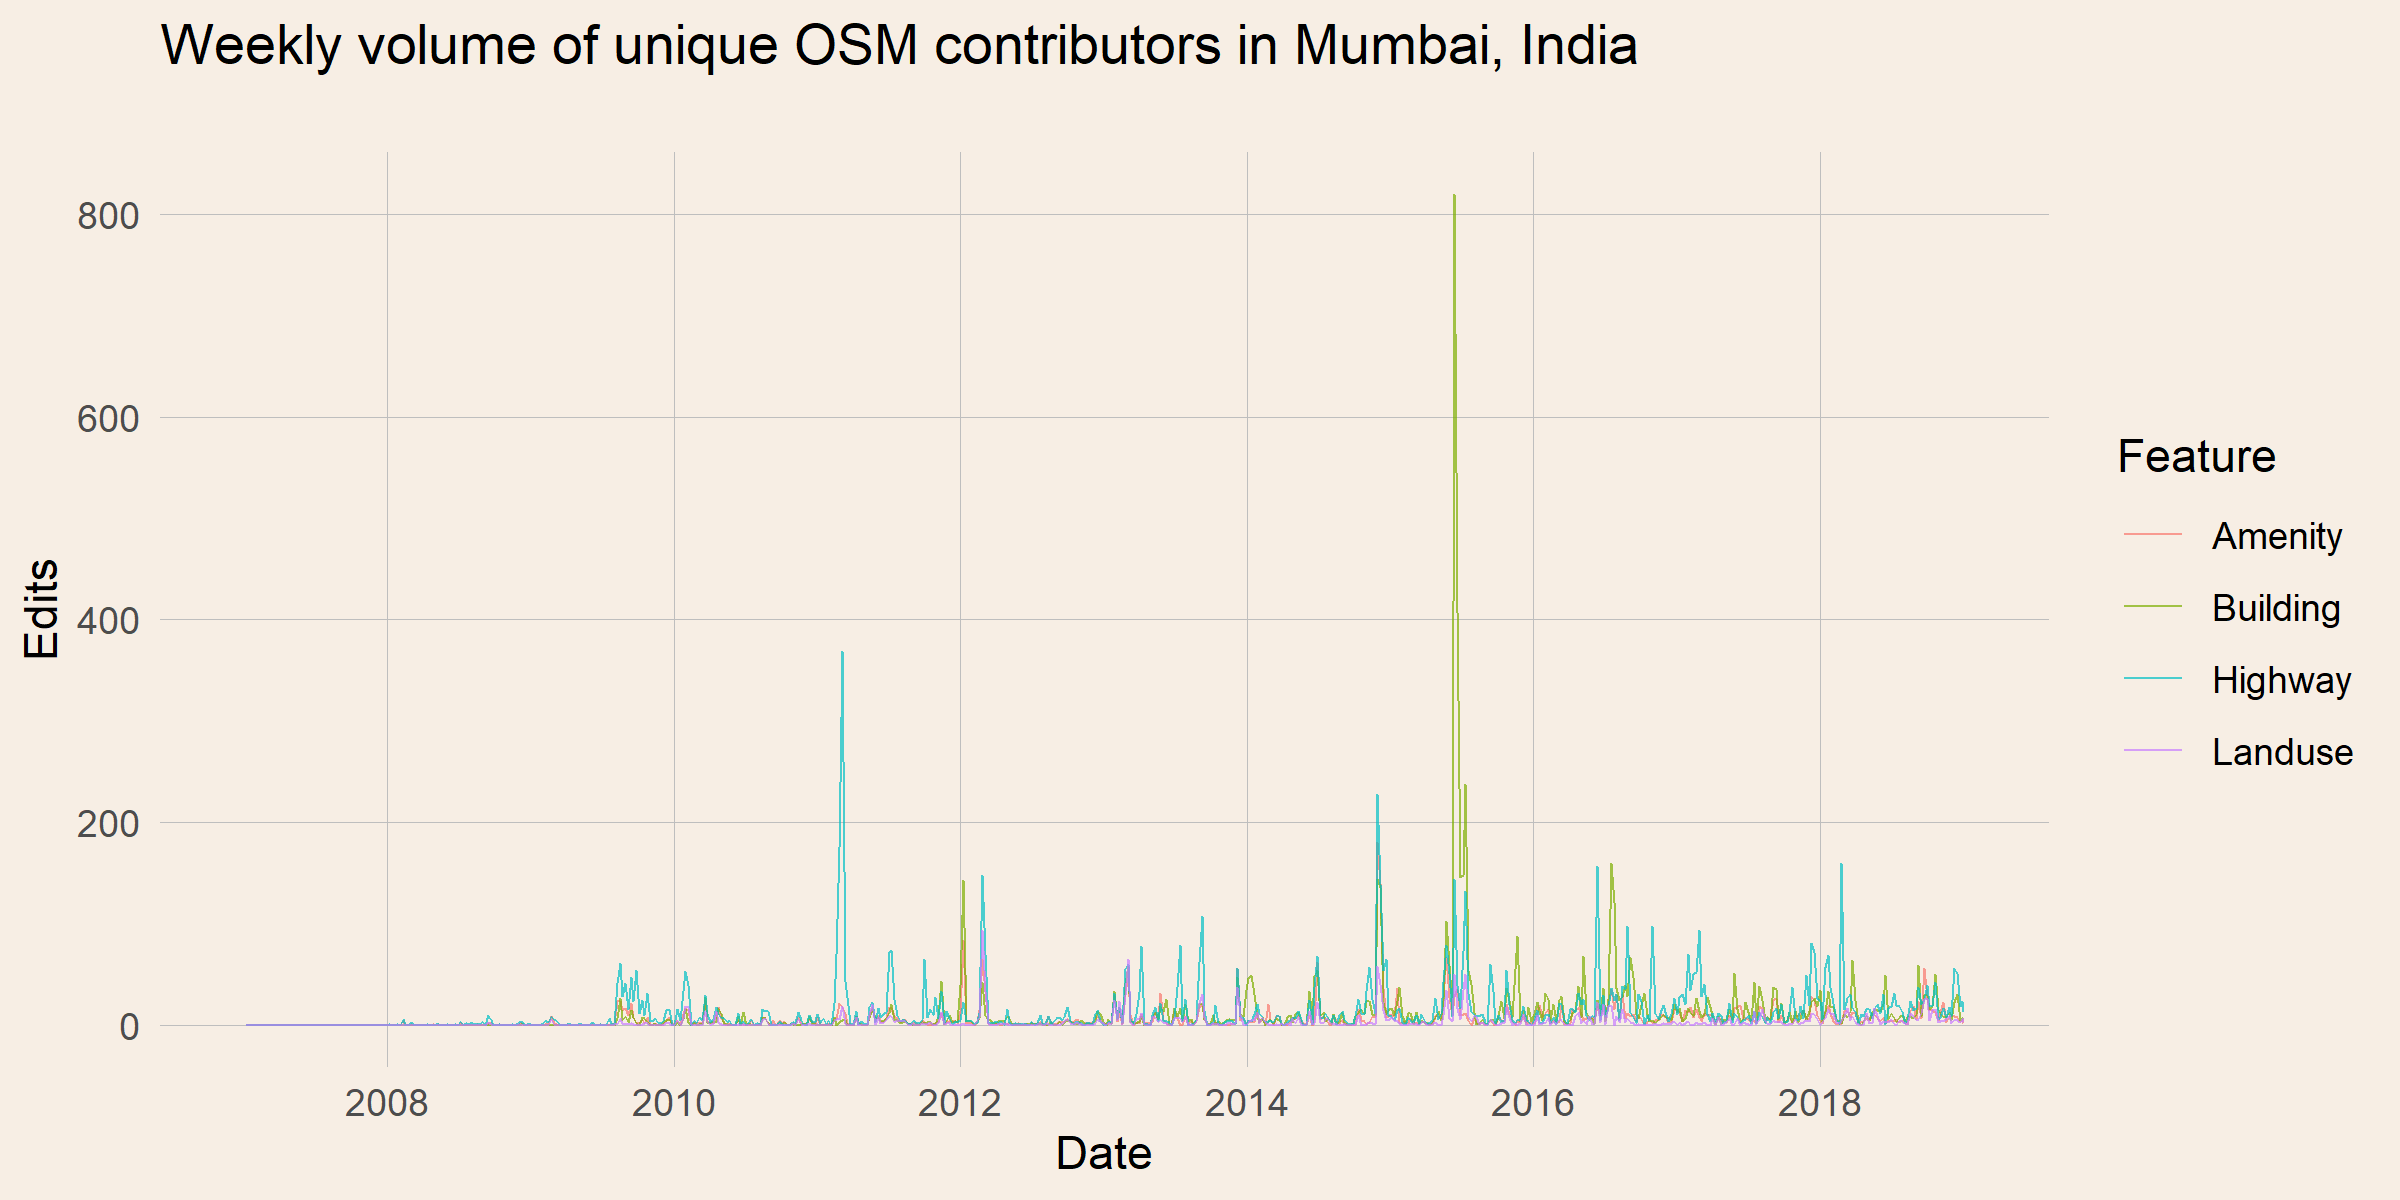
\includegraphics[width = \textwidth]{Images/mb_users_agg.png} %this tells latex what graphics to include. I put my images in an 'Images' folder to aid file management, hence the Images/ before the file name. the width bit before allows you to alter the width of the image. It is also possible to use scale as well as using equations with the textwidth to make it say half the text width.
    \caption{This is an example image} % this prints the caption below the figure
    \label{fig:four} % this internally labels the figure for future referencing.
\end{figure}

These unique modes of data production, considered over time, have important implications for the temporal accuracy of the data. 

\section{Sample formatting}

\textbf{this is bold text} and \textit{this is italicized text}. ctrl b and ctrl i work as shortcuts. 

Create an ordered list 

\begin{enumerate}
    \item Enumerate
    \item lists
    \item look
    \item like
    \item this.
\end{enumerate}

Create an unordered list 

\begin{itemize}
    \item Itemize
    \item lists
    \item look
    \item like
    \item this.
\end{itemize}

Create a nested list 

\begin{enumerate}
    \item Wow
    \begin{enumerate}
        \item another
        \begin{enumerate}
            \item nested
            \begin{enumerate}
                \item list
            \end{enumerate}
        \end{enumerate}
    \end{enumerate}
\end{enumerate}